\documentclass[main.tex]{subfiles}

\begin{document}

\section{Issue #2557}
\label{sec:2557}

When typing display math LaTeX in a markdown note, the written LaTeX is parsed correctly but displayed incorrectly, with certain constructs having line breaks between tokens.

\subsection{Steps}
\label{subsec:steps2557}

\begin{enumerate}
\item Launch Boostnote
\item Open a new Markdown Note. Press \textit{Ctrl N} or click on the icon next to the search bar; then select Markdown Note.
\item Toggle mode to two panels in the top right corner (should be the default). Now you should have two panels open, the edit and view panels.
\item Reproduce the error. Type the following in the edit panel:
\end{enumerate}

\begin{verbatim}
        $$
        \begin{aligned}
           &P(X=x)=\binom{n}{k}P^x(1-p)^{(n-x)}\\
           &Var(X)=np(1-p)
        \end{aligned}
        $$
\end{verbatim}

\subsection{Requirements}
\label{subsec:req2557}

As of release v0.11.9 of Sep 9, and upstream master branch as of Nov 14, we get this result:

\begin{figure}[h]
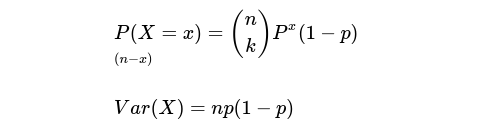
\includegraphics[scale=0.6]{images/bug1.png}
\centering
\end{figure}

However, the expected result is naturally:

\begin{figure}[h]

\includegraphics[scale=0.6]{images/bug2.png}
\centering
\end{figure}

The problem is that there is a line break where there should not be one: line breaks in display math mode are not allowed outside environments, and inside environment aligned line breaks are inserted with '\textbackslash\textbackslash', enumerating equations.

\subsection{Source Code Files}

The bug is the file:

\begin{itemize}
\item  browser/components/markdown.styl
\end{itemize}

\begin{figure}[h]
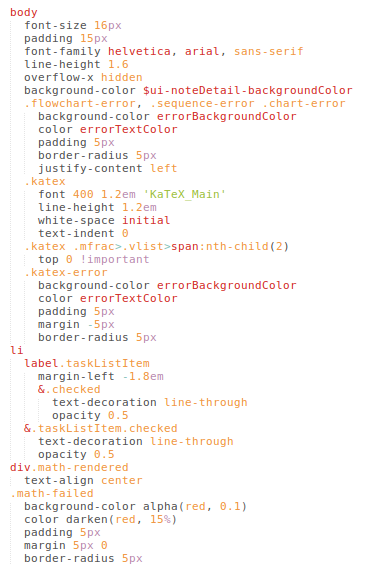
\includegraphics[scale=0.6]{images/code.png}
\centering
\end{figure}

\subsection{Source of the problem}

The problem is not in the dependency (\textbf{KaTeX}). The \textbf{KaTeX} dependency includes its own major stylesheet, which should enforce this restriction on its own display math elements. So the problem should be in some of Boostnote's own style sheets, conflicting somehow with those of \textbf{KaTeX}.

Inspecting the elements inside Boostnote (\textit{Ctrl Shift I}) suggests looking at class names \textit{.katex} and \textit{.katex-display}, as the rendered LaTeX parent element has these class names. A quick

\begin{verbatim}
        grep -rnE "\\.katex" browser/
\end{verbatim}

immediately pinpoints file markdown.styl.

\subsection{System Architecture}

A simple rundown of Boostnote's main dependencies, with emphasis on markdown-it and katex:

\begin{figure}[h]
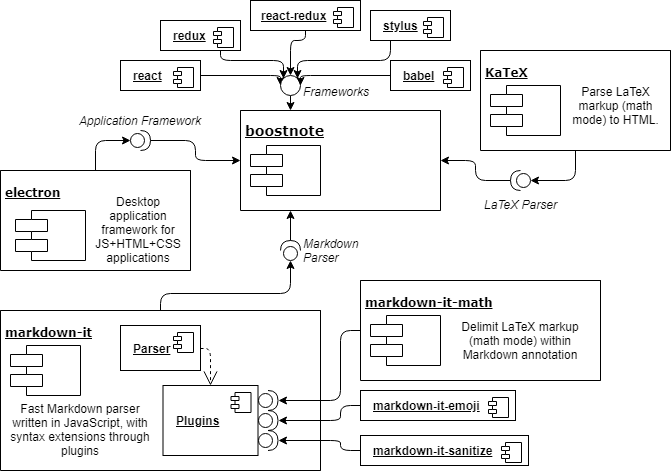
\includegraphics[scale=0.6]{images/diagram.png}
\centering
\end{figure}

\subsection{Design of the fix}

\textbf{Discussion}\\

KaTeX, being a LaTeX formatting engine for the web, would certainly not have made it this far while allowing line breaks inside display math environments generally. We verified this earlier. So Boostnote's own stylesheets must be messing around where they shouldn't, and overwriting KaTeX's imported stylesheets.

There are a few ways to fix this issue, but a proper fix will ultimately be a \textbf{breaking change} as it will disallow line wrapping in display math environments --- much to the dislike of some users, probably.

Changing this attribute to nowrap will have unintended side effects (no wrapping in inline math mode), so the problem, albeit simple, will require further testing. The most likely solution will involve demoting selector body .katex to .katex-inline or removing the attribute, or even removing the .katex rules altogether.\\

\textbf{Source of the problem}\\

The problem is not in the dependency (KaTeX), see \href{https://github.com/KaTeX/KaTeX/issues/1732}{this discussion}. The KaTeX dependency includes its own major stylesheet, which should enforce this restriction on its own display math elements.

Inspecting the elements inside Boostnote (Ctrl Shift I) suggests looking at class names .katex and .katex-display, as the rendered LaTeX parent element has these class names. A quick

\begin{lstlisting}
    grep -rnE "\\.katex" browser/
\end{lstlisting}

on the repository's main directory immediately pinpoints file \textbf{browser/components/markdown.styl}.

At \href{https://katex.org/}{katex.org} we compare the computed styles of the LaTeX shown on the front page to those of Boostnote applied to the same LaTeX elements. In particular we looked at attributes like display, textalign, and overflow-wrap. We concluded quickly that the problem was in the attribute \textit{white-space}, whose value was reset to \textbf{initial} in Boostnote (in this case normal) for everything math element, instead of \textit{nowrap} which is KaTeX's own style.

\subsection{Fix source code}

The fix is essentially removing style *whitespace nowrap" from \textit{markdown.styl} while causing the smallest possible breaking change. After due analysis and experimentation on a variety of LaTeX constructs we decided to remove the entire rule \textit{.katex} and replace it with a simple switch: \textit{whitespace nowrap} for KaTeX display elements and \textit{whitespace initial} otherwise.

\subsection{Validate the fix}

\textbf{Solution Images}

Consider the following content of a Markdown Note, containing mostly LaTeX and little Markdown:

\begin{figure}[H]
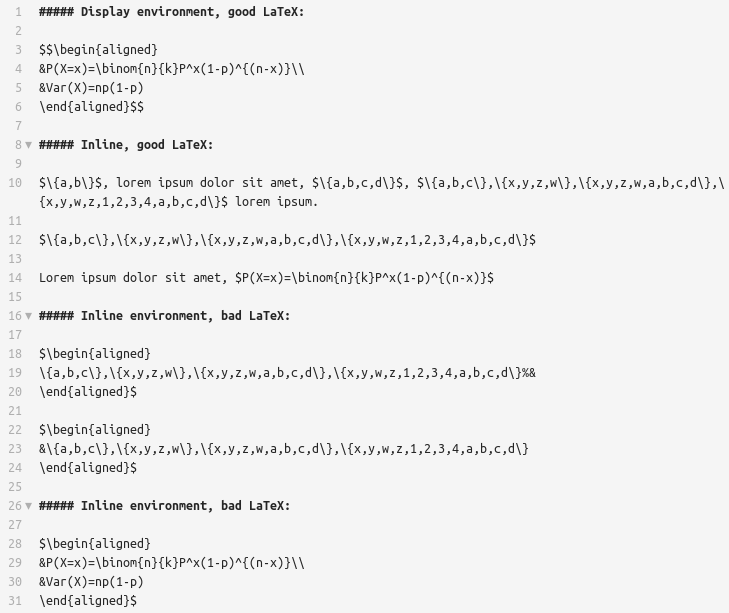
\includegraphics[scale=0.5]{images/solution1.png}
\centering
\end{figure}

Now, below on the left is Boostnote's representation of the above LaTeX, and on the right that same LaTeX after the fix.

\begin{figure}[H]
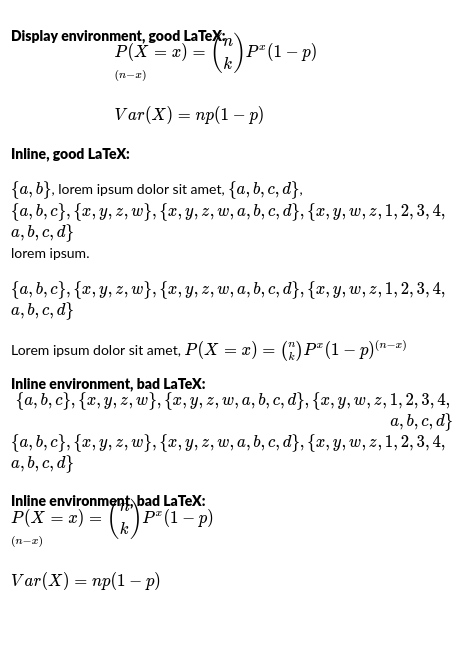
\includegraphics[scale=0.40]{images/solution2.png}
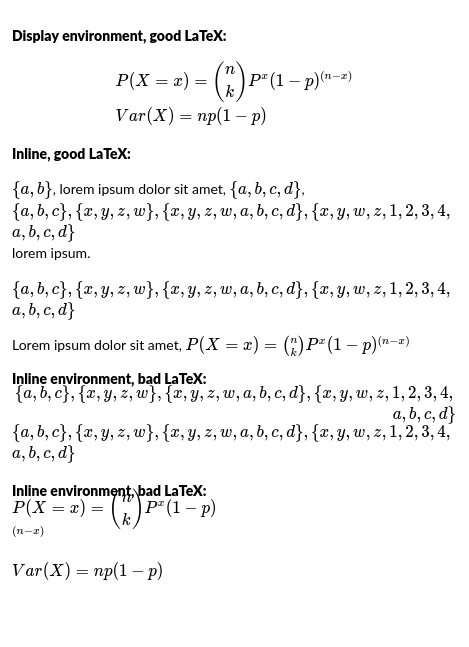
\includegraphics[scale=0.40]{images/solution3.png}
\centering
\end{figure}

\begin{figure}[H]
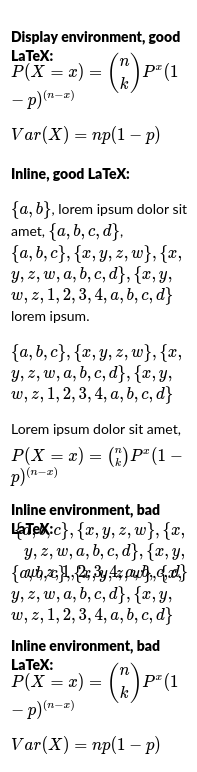
\includegraphics[scale=0.43]{images/solution5.png}
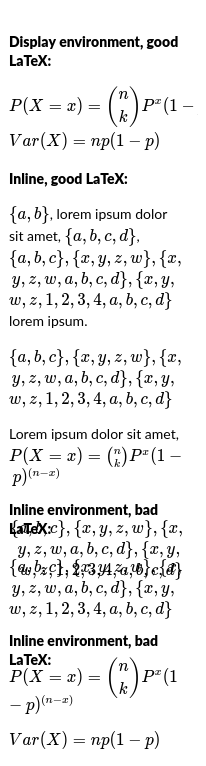
\includegraphics[scale=0.43]{images/solution6.png}
\centering
\end{figure}

Notice how, on the narrow display panel, the display math overflows the x-axis and is hidden. This is the expected behaviour in any LaTeX document.

\subsection{Submission of the fix}

The pull request was accepted on 16 December.

The issue was not changed from Delivery #1, nor any extra/adjacent issues were created or fixed along with this one.

\section{Wrap Up}

Diogo Yaguas - Searching issues and report

Bruno Carvalho - Issue \#2557

Tiago Castro - Issue \#2554\\

The work distribution was equally distributed.

\nocite{*}

\end{document}